\chapter{Methods}
\section{Finding the steady states: Newton-Raphson method}\label{newton_raphson}

To obtain the roots of the system, the Newton-Raphson algorithm was implemented.
The Newton-Raphson algorithm, also known as Newton's method, is a numerical technique for finding approximate roots of a real-valued function. It starts with an initial guess, which is then refined through iterations. In each iteration, the method uses the current approximation to find a better one, applying the formula
\begin{equation}
x_{n+1} = x_{n} - \frac{f(x_{n})}{f'(x_{n})}
\end{equation}

where $f(x)$ is the function and $f'(x)$ its derivative.

This algorithm was implemented in Python using a tolerance value of $10^{-6}$ and a maximum of 15 iterations after which the algorithm stopped searching for a root.
Because the system had the potential for multi-stability, several initial conditions need to be searched to obtain all steady states.
In total 100 initial conditions were analysed by the Newton-Raphson to obtain all the roots of the system.
The 100 conditions were sampled with Latin-hypercube sampling of a $n$ dimensional space ($n$ being the number of species), from a uniform distribution with a range from $10^{-3}$ and $10^3$.
\section{Sampling method}\label{sampling method}
If no parameters from a system are known, sampling of the whole parameter space must be done to understand the system's behaviour.
Different methods exist for sampling parameter spaces.
Several studies have shown that Latin-hypercube sampling (LHS) has a higher efficiency than grid sampling or random sampling when searching through high-dimensional spaces.
The efficiency of LHS over grid sampling might be explained because not all dimensions of the model are important, meaning some parameters might be sloppy.
Therefore, not all parameters have to be explored thoroughly as done in grid sampling~\parencite{Iman2014, Bergstra2012}.
The three sampling regimes are shown in Fig.~\ref{fig:distributions}A.

In LHS, a distribution and a number of desired samples are given as an input.
The algorithm then divides the space sections according to the distribution given (e.g. in a normal distribution, more sections will appear near the mean value).
Then, one sample is positioned randomly somewhere in each section.
For a 2-dimensional parameter space, no samples can be in the same column or row.
This can be scaled up to high multidimensional spaces.
The LHS scheme is shown in Fig.~\ref{fig:distributions}B.
\begin{figure}[H]

    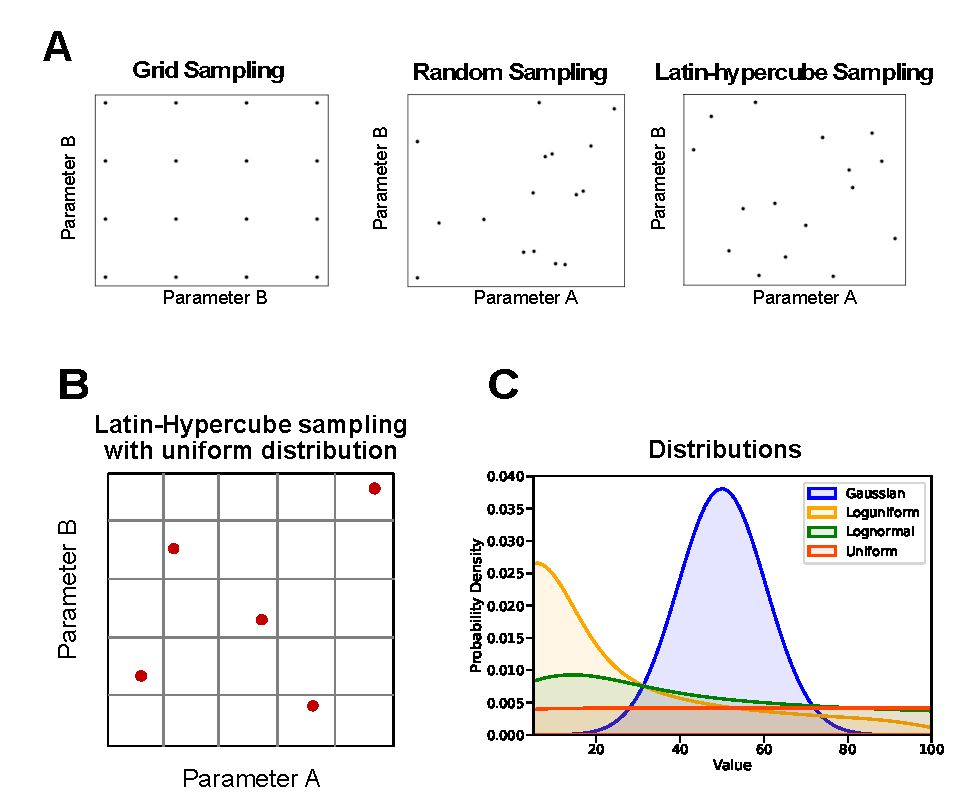
\includegraphics[width=1\textwidth]{chapters/Methods/distributions}
    \caption{\textbf{Sampling method for high dimensional spaces}. \textbf{(A)} Types of potential sampling methods. \textbf{(B)} Latin-Hypercube sampling with uniform distribution for a 2-dimensional parameter space. Space is separated into 5 sections for each parameter, leading to 5 samples (red dot). No sample is present in the same row or column. \textbf{(C)} Parameter distributions used for Latin-hypercube sampling. The four different types of parameters have different distributions depending on the ranges defined. All of them are uniform distributions on a log scale.}
    \label{fig:distributions}
\end{figure}
The distribution given as an input to the LHS algorithm will be the resulting distribution of your samples.
For this search, several distributions are chosen (Fig.~\ref{fig:distributions}C).
Amongst those, we commonly use the uniform distributions in a logarithmic scale (log-uniform distribution).
The uniform distribution, although it does not describe many phenomena in biology, can be useful when no prior knowledge is known about the parameters~\parencite{Frank2009}.
The logarithmic component is used to make sure parameters from all scales are represented equally, instead of having a higher frequency of values from larger scales.
Log-normal distributions are commonly used for modelling in biology, however, due to the nonexistent prior knowledge on our parameter values, the log-uniform is used instead.
When we have some level of certainty about a parameter, a Gaussian distribution is used.
Finally, if we are completely sure, a fixed distribution is used.

\section{PostgreSql database}\label{PostgreSql database}
A PostgreSQL was created from scratch to store and organise all the linear stability analysis and numerical results.
This schema is composed of 5 tables as seen in Fig.~\ref{psql_schema}.
Model parameters and Simulation parameters have information on the kinetic parameters of the model and the simulation parameters of the numerical solver.
A set of model parameters or simulation parameters is encoded with a primary key for each table: model\_param\_id and sim\_param\_id.
LSA output contains information on the linear stability analysis output for a specific model\_param\_id.
This information involves the type of dispersion relation, the highest eigenvalue, the LSA estimated wavelength...etc.
Simulation output contains information on the 1D or 2D time-series data obtained from the simulation. Each set of data has a model\_param\_id and a sim\_param\_id associated to it.
Finally, the Pattern type table has information on the type of pattern of a specific numerical output.
This is based on the defined classifications (e.g. convergence, spatial homogeneity and number of peaks).
As with the Simulation output table, each data point has a model\_param\_id and a sim\_param\_id associated to it.

This method enables the understanding of relationships between numerical and analytical outputs and between different types of solutions.
Additionally, it creates a safe and documented way to store all results in an organised manner.

\begin{figure}[H]

    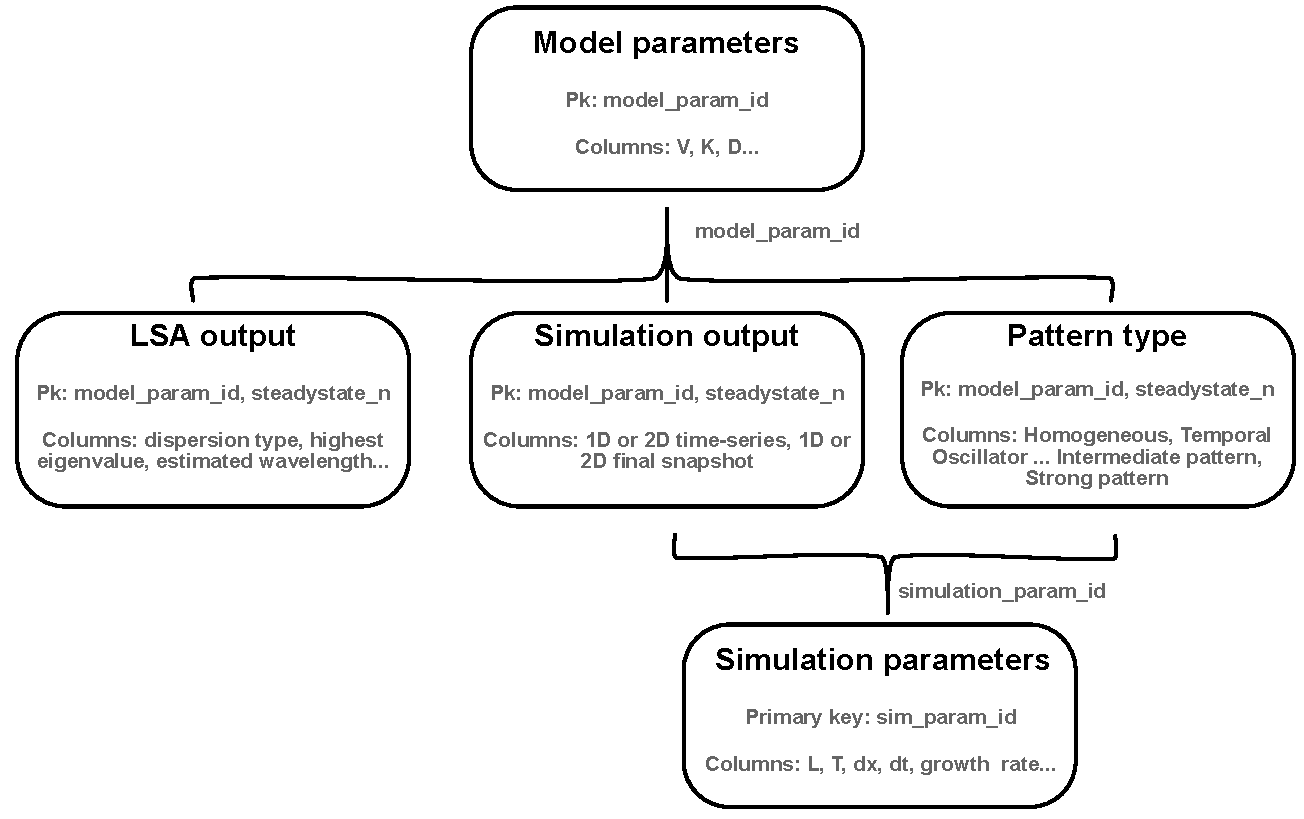
\includegraphics[width=1\textwidth]{chapters/Methods/psql_schema}
    \caption{\textbf{PostgreSQL database schema}}
    \label{psql_schema}
\end{figure}

\section{Wavelength and convergence time from numerical data}\label{Wavelength and convergence time from numerical data}
The wavelength was obtained by computing the average distance between peaks in the solution.
A wavelength is found for every species of the model, which in the case of Chapter~\ref{Chapter 1} is 2 species.
Then the average between the various wavelengths (which are expected to be similar) is computed.
The average is found using the \textit{findpeaks} package in Python with all the default parameters and a prominence of 0.5.

The convergence time is obtained by testing when in time the pattern stops being converged starting from the end.
A pattern will be considered converged if the last 30 time points for any of the two molecular species fulfils the following condition
\begin{equation}
    \frac{max(U[-30:]) - min(U[-30:])}{max(U[-30:])} \leq 0.05
\end{equation}

\section{Dispersion peak height optimisation: Adapted random walk Metropolis}\label{dispersion_peak_optimisation}
In this section, the optimisation of the dispersion peak height using an adapted random walk-metropolis (RWM) algorithm will be explained.
The RWM algorithm is a common type of Markov Chain Monte Carlo (MCMC) method that uses a Metropolis Algorithm.
The RWM algorithm sampled from the posterior distribution, without getting stuck in local maxima.
This algorithm is used in a Bayesian context when trying to fit a model with parameters $\theta$ to data $D$.
A probability distribution is obtained, which suggests what parameters $\theta$ are better to represent the data $D$.
However, in this case, the aim is not to fit a model to any data $D$ but to maximise the dispersion peak height.
Therefore, a variant of the RWM algorithm will be developed as shown in Fig.~\ref{Simulated Annealing}.

\begin{figure}[H]
    \centering
    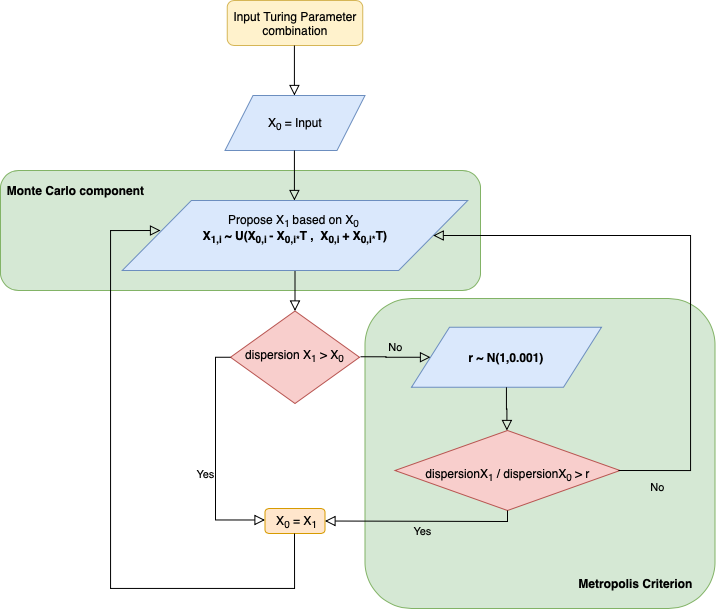
\includegraphics[width=1\textwidth]{chapters/Methods/Simulated Annealing}
    \caption{\textbf{Adapted random walk-Metropolis algorithm workflow}.  }
    \label{Simulated Annealing}
\end{figure}

The starting point of the algorithm is to propose a Turing parameter set which will be the starting parameter set to be optimized in the process.
From that parameter set, a new parameter set is proposed where all parameters are varied slightly.
The variation is chosen randomly from a uniform distribution around the parameter value.
The uniform distribution is defined as $U(X_{0} - X_{0}T, X_{0} + X_{0}T)$, where $X_{0}$ is the initial parameter to be varied and T is a temperature constant that will define the amount of variation to be applied.
In this case, $T=0.1$.
In this case, $T=0.1$.
So if $X_{0}=100$, the uniform distribution is U(90,110).
This step is done for all parameters of the parameter set at every iteration, producing a new parameter set $X_{1}$.
The Markov Chain component is present because the step taken is only dependent on the current state, and not on information prior to that.
The Monte Carlo is due to the randomness involved in choosing the new parameter set.
In the normal RWM algorithm, the posterior of $X_{0}$ and $X_{1}$ are compared to see which parameter set is a better fit to the data $D$.
However, for the purpose of optimising dispersion, the posterior is neither available nor relevant.
Instead, the dispersion peak height value is used.
Once the new step $X_{1}$ is taken, the dispersion peak height ($d_{X_{1}}$) is calculated and compared to the dispersion peak height of $X_{0}$ ($d_{X_{0}}$). If the dispersion peak height has improved, $d_{X_{1}} > d_{X_{0}}$, the move is accepted and $X_{1}$ becomes $X_{0}$.
If no improvement has been made, $d_{X_{1}} < d_{X_{0}}$, the Metropolis algorithm comes into place: The ratio of the dispersions is calculated, $r = \frac{d_{X_{1}}}{d_{X_{0}}}$ and compared to a normal distribution $N(1,0.001)$.
If the ratio is higher than a random number from the distribution $N(1,0.001)$, the move is accepted and $X_{1}$ becomes $X_{0}$.
Otherwise, the move is rejected.
This ensures that big decreases in the dispersion peak height ($r \ll 1$) are less likely to be accepted than small decreases ($r \approx 1$).
Usually, the RWM uses a distribution $U(0,1)$ for this step.
An optimization with this distribution was attempted, resulting in no significant improvement of the dispersion peak height.
Therefore, the variant of the $N(1,0.001) $ was introduced to ensure a more strict regime is in place, hence reducing the number of accepted negative steps.


\section{Numerical solution by finite-difference methods}\label{numerical_methods}
Obtaining a solution for a system of equations can become a complex problem if working with a large system of non-linear PDEs.
Because an analytical expression for the solution is almost impossible to obtain, finite-difference methods are used for cases like this one.
Finite-difference methods consist of discretising space and time to approximate the PDE system to a system of algebraic equations that can be easily solved by matrix algebra techniques~\parencite{Morton1994}.
By discretising time and space, the two independent variables can be expressed as:
\begin{subequations}
    \begin{equation}
        t_{n} = n \cdot \Delta t, \quad n=0,\dots,N-1
    \end{equation}
    \begin{equation}
        x_{j} = j \cdot \Delta x, \quad j=0, \dots,J-1
    \end{equation}
\end{subequations}
While $\Delta t$ and $\Delta x$ are the time steps and the space steps respectively, N and J are the number of discrete time and space points in our grid.
$\Delta t$ and $\Delta x$ can be defined as $ \Delta t = \frac{T}{N}$ and $\Delta x= \frac{L}{J}$ respectively where T and L are the final time and space values in the grid.
The aim is to derive a numerical solution that approximates the unknown analytical solution so $U(j\Delta x, n\Delta t)\approx u( j\Delta x, n\Delta t)$, where $U$ is the analytical solution and $u$ is the numerical solution.

When working with a numerical solver, the solver can perturb the system behaviour due to the effects of the time-step, the integration method or the computer arithmetic.
When choosing a scheme to numerically solve a PDE, three different characteristics of the scheme need to be considered: Consistency, stability and convergence.
Firstly, for a scheme to be consistent, the truncation error must be reduced as $\Delta t \rightarrow 0$ or/and if $\Delta x \rightarrow 0$.
The truncation error results from using a simple approximation to represent an exact mathematical formula.
Secondly, the numerical method is said to be stable if the error (truncation or round-off) is not magnified as the number of time steps tends to infinity.
Finally, as the Lax equivalence theorem states, the scheme is said to be convergent if both consistency and stability are fulfilled.
This means that at any fixed point, if time and space discretisations tend to zero, the numerical solution will tend towards the exact solution~\parencite{smith1985numerical}.
The methods chosen to solve this system of equations are \acrfull{CN} for 1 dimension in space and \acrfull{ADI} for 2 dimensions. These methods are chosen because they are both unconditionally stable as shown by von Neumann stability analysis~\parencite{strikwerda2004finite}. The unconditional stability is important to allow for larger $\Delta t$ and $\Delta x$, without getting an amplification of the error. Larger $\Delta t$ and $\Delta x$ will result in reduced computational power. Although \acrshort{CN} is less computationally expensive than \acrshort{ADI}, it becomes extremely complex when scaled up to multiple dimensions. On the other hand, \acrshort{ADI} has a simpler structure in 2 dimensions that can be solved easily using the tridiagonal matrix algorithm. Hence, \acrshort{CN} is used to obtain 1D space solutions while \acrshort{ADI} is used for 2D.
\begin{figure}[H]

    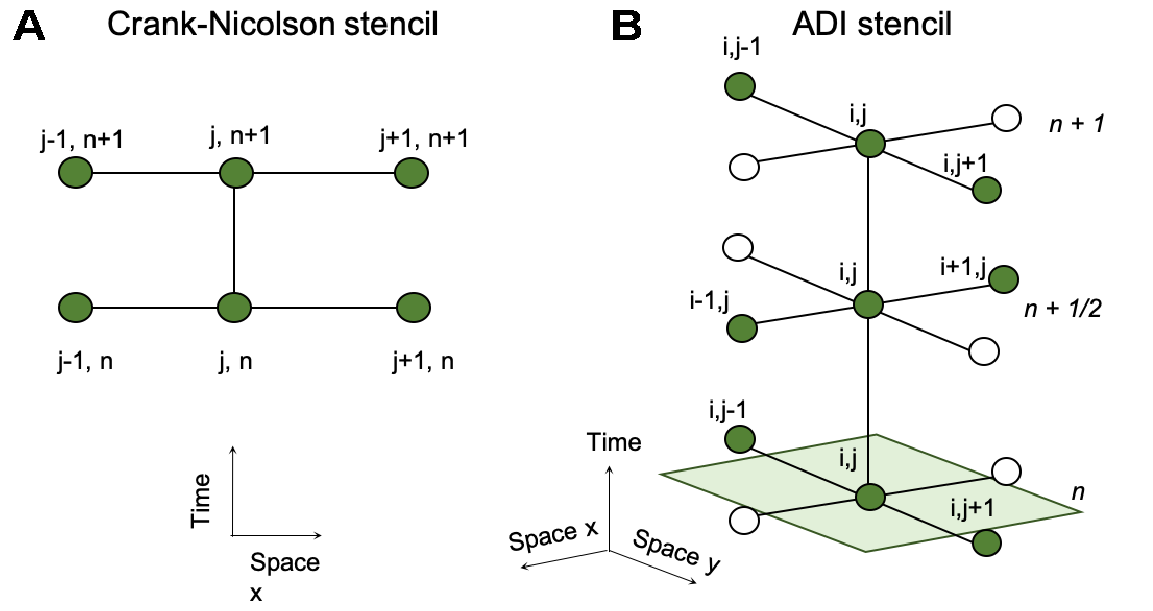
\includegraphics[width=1\textwidth]{chapters/Methods/stencils}
    \caption{\textbf{Stencils for numerical solution}.  A stencil is a geometric representation with nodes and edges, that represents the points of interest for the numerical approximation. The points of interest, which are the ones present in the equations, are shown in green. j and n are the current space and time points. \textbf{(A)} \acrlong{CN} stencil used in 1D numerical simulations. The axes are time and space ($x$). \textbf{(B)} \acrshort{ADI} stencil used in 2D numerical simulations. The axes are time and 2D space ($x$,$y$).}
    \label{fig:stencils}
\end{figure}


\subsection{Crank Nicolson Method}\label{cranknicolson}
Consider a reaction-diffusion system with one space dimension
\begin{equation}
    \frac{\delta u}{\delta t} =  f(u) + D\pdvn{2}{u}{x}
\end{equation}
The spatial part of the equation can be approximated to
\begin{equation}
    \pdvn{2}{u}{x} \biggr\rvert_{x=j\Delta x,t=n\Delta t} \approx \frac{1}{2\Delta x^{2}}\left( U^{n}_{j+1} -  2U^{n}_{j} + U^{n}_{j-1} + U^{n+1}_{j+1} - 2U^{n+1}_{j} + U^{n+1}_{j-1}\right),
\end{equation}
while the production function can be approximated to $f ( U^{n}_{j})$.  The approximations can be better visualised using the \acrshort{CN} stencil (See Fig.\ref{fig:stencils}a).
Applying \acrshort{CN} stencil to the grid point (i,j), the reaction-diffusion system can be expressed as

\begin{equation}
    \frac{U^{n+1}_{j} - U^{n}_{j}}{\Delta t} = \frac{D}{2\Delta x^{2}}\left( U^{n}_{j+1} -  2U^{n}_{j} + U^{n}_{j-1} + U^{n+1}_{j+1} - 2U^{n+1}_{j} + U^{n+1}_{j-1}\right) +  f( U^{n}_{j})
    \label{CN_stencil}
\end{equation}
By reordering this approximation into a linear equation, the resulting problem is defined by a simple linear equation containing matrices A and B. Where $\textbf{U}^{n+1} = [U^{n}_{0}, \ldots , U^{n}_{J-1}]$, the simplified system can be expressed as:
\begin{equation}
    \textbf{U}^{n+1} = A^{-1}(B\textbf{U}^{n} + f^{n})
\end{equation}
This method simplifies the complex system into a linear system that can be solved numerically. The solution given will be a 1D space solution of the reaction-diffusion system. Although the method is unconditionally stable, the solution can contain oscillations if $ \frac{\Delta t}{\Delta x^{2}} >\frac{1}{2} $ \parencite{trefethen1996finite}. Therefore, the ratio will be kept below $\frac{1}{2}$ to avoid errors.

\subsubsection{Introducing Dirichlet or absorbing boundary conditions}\label{methods_boundary_conditions_CN}
CN method can be implemented with Neumann no-flux boundary conditions or Dirichlet absorbing boundary conditions.
For Neumann no-flux boundary conditions:
\begin{equation}
    \frac{\delta u}{\delta t} =  f(u) + D\pdvn{2}{u}{x},   \quad \quad \quad \quad \quad \quad \pdv{u}{x}\biggr\rvert_{x=0,L}=0
\end{equation}

the values of $U_{j}$ at $j=0$ and $j=J-1$ are

\begin{equation}
    U_{j=0} = U_{j=-1}  \quad \quad \&  \quad \quad  U_{j=J-1} = U_{j=J}
\end{equation}

These value of $U_{j=0}$ and  $U_{j=J-1}$ is replaced into the CN stencil shown in Eq.~\ref{CN_stencil}.
These values are chosen to ensure the derivative at the boundary is zero.

Similarly, Dirichlet absorbing boundary conditions are represented by the following system

\begin{equation}
    \frac{\delta u}{\delta t} =  f(u) + D\pdvn{2}{u}{x},   \quad \quad \quad \quad \quad \quad U\biggr\rvert_{x=0,L}=0
\end{equation}

and have values of $U_{j}$ at $j=-1$ and $j=J$ such as

\begin{equation}
    U_{j=-1} = 0  \quad \quad \&  \quad \quad  U_{j=J} = 0
\end{equation}

These values of $U_{j=0}$ and  $U_{j=J-1}$ is replaced into the CN stencil shown in Eq.~\ref{CN_stencil}.
These values are chosen to ensure the value at the boundary is zero.



\subsection{Alternating Direction Implicit Method}\label{ADI}
As done in the \acrshort{CN} scheme, a reaction-diffusion system and its boundary conditions will be considered. However, in this case, two spatial dimensions will be introduced.

\begin{equation}
    \frac{\delta u}{\delta t} =  f(u) + D\left(\pdvn{2}{u}{x} + \pdvn{2}{u}{y}\right) ,   \quad \quad \quad \quad \quad \quad \pdv{u}{x}\biggr\rvert_{x=0,L}=0 \quad \quad \pdv{u}{y}\biggr\rvert_{y=0,L}=0
\end{equation}
If the CN stencil is applied to this 2D spatial problem, the system would contain banded matrices on the right and left-hand sides, which would be very expensive to invert. \acrshort{ADI} offers an alternative in which tridiagonal matrices are inverted instead of banded matrices (less computational power required). The characteristic of \acrshort{ADI} is the time step $\Delta t$ is split into two, and each half-time step is computed. This means, that to compute the change at each time step, first we compute $U^{n+1/2}_{i,j} $ and from there,    $U^{n+1}_{i,j} $ is calculated. This results in two different equations:
\begin{subequations}
    \begin{equation}
        \begin{split}
            \frac{U^{n+1/2}_{i,j} - U^{n}_{i,j}}{\Delta t/2} = \frac{D}{2\Delta x^{2}}\left( U^{n+1/2}_{i+1,j} -  2U^{n+1/2}_{i,j} + U^{n+1/2}_{i-1,j}\right)  \\+ \frac{D}{2\Delta y^{2}}\left( U^{n}_{i,j+1} -  2U^{n}_{i,j} + U^{n}_{i,j-1}\right)  + \Delta t f(U^{n}_{i,j})
        \end{split}
    \end{equation}
    \begin{equation}
        \begin{split}
            \frac{U^{n+1}_{i,j} - U^{n}_{i,j}}{\Delta t/2} = \frac{D}{2\Delta x^{2}}\left( U^{n+1/2}_{i+1,j} -  2U^{n+1/2}_{i,j} + U^{n+1/2}_{i-1,j}\right)  \\+ \frac{D}{2\Delta y^{2}}\left( U^{n+1}_{i,j+1} -  2U^{n+1}_{i,j} + U^{n+1}_{i,j-1}\right)  + \Delta t f(U^{n+1/2}_{i,j})
        \end{split}
    \end{equation}
\end{subequations}
In the first half-time step (Equation 46a), the $x$ derivative is taken implicitly, and in the second half-time step (Equation 46b), the $y$ derivative is taken implicitly. As done in \acrshort{CN}, the approximation is reordered into a linear system. Two families of linear systems appear:
\begin{subequations}
    \begin{equation}
        A\textbf{U}^{n+1/2}_{x,i} = \textbf{b}_{i} + \textbf{f}(\Delta t \textbf{U}^{n}_{x,i}), \quad i=0,\ldots,I-1
    \end{equation}
    \begin{equation}
        C\textbf{U}^{n+1}_{y,j} = \textbf{d}_{j} + \textbf{f}(\Delta t \textbf{U}^{n+1/2}_{y,j}), \quad j=0,\ldots,J-1
    \end{equation}
\end{subequations}
Again, this method also simplifies a complex system into a linear system that can be solved numerically, as in \acrshort{CN}. However, this method allows for the introduction of a new spatial dimension and therefore produces a 2D spatial solution. The workings of this method can be better understood with the \acrshort{ADI} stencil (See Fig.~\ref{fig:stencils}b). \acrshort{ADI} will be used to visualise patterns in 2D.


\subsubsection{Introducing Dirichlet or absorbing boundary conditions}\label{methods_boundary_conditions_ADI}
As with the CN method, ADI can also be implemented with Neumann no-flux boundary conditions or Dirichlet absorbing boundary conditions.
The implementation is the same as in CN (See Section~\ref{methods_boundary_conditions_CN}).
However, in this case, boundaries are considered for both $i$ and $j$, both in steps $U^n$ and $U^{n+1/2}$.

\subsection{Analysis of numerical solution}
The speed of pattern formation and pattern wavelength are identified by performing additional analysis on the 1D numerical data.  \\\\
\subsubsection{Time for pattern convergence}
The development of the pattern follows a certain behaviour: The molecule concentrations are initially homogeneous; then a pattern gets formed progressively; and finally, the pattern is in its final state and the solution remains constant.
The time for pattern convergence is measured by comparing the solution (one point in space) at every time point to the solution at the final time point. If the difference is smaller than a tolerance value of $10^{-4}$ that time point is taken as the convergence time point where the pattern has finished to develop. \\\\
\subsubsection{Wavelength prediction from numerical solution}
The findpeaks package is used from the \textit{scipy.signal} Python library. All peaks in the final time point of the 1D simulation are found through the findpeaks package. The average distance between peaks is taken and that distance is averaged throughout the 6 species.

\section{Image recognition and modelling for confocal microscopy data}
\subsection{Tissue area recognition}\label{Tissue area recognition}
From a confocal microscopy image, we want to obtain the shape of the biofilm.
The image is opened and processed using the PIL package in Python.
After splitting the image into RGB, the blue channel is selected.
Because the cells show red and green fluorescence, the blue channel is minimal in the tissue compared to the agar.
A Gaussian filter is used to smooth the image and get a continuous biofilm.
Blue channel pixels with values above a threshold (20) are selected and fixed to 0 in the "shape matrix".
The rest of the pixels are set to 1 which determine the area of the biofilm.

\subsection{Plotting superposed numerical solution as confocal microscopy results}\label{Plotting superposed numerical solution as confocal microscopy results}
To compare the model and experiments, the six variable solutions steaming from the six-equation model have to be translated into the red-green superposed images obtained from the confocal microscopy.
The red and green channels are obtained from the solutions of species D (LacI) and E (cI*), which are assumed to have a linear relationship with GFP and mCherry respectively (Eq~\ref{linear_fluorescence}) through parameter $\alpha$.
These two channels are transformed using min-max scaling to range from 0-255:

\begin{equation}
    X_{scaled} = \frac{x-x_{min}}{x_{max}-x_{min}} \cdot 255
\end{equation}

This way, we end up with a red and green channel ranging from 0-255 (Fig.~\ref{redgreesupersposed}A,B).
This can be plotted as an RGB image where the blue channel is zero (Fig.~\ref{redgreesupersposed}C).
This normalisation also occurs when adjusting the gain for each fluorophore during the confocal microscopy.
Therefore, as long as the linear relationship between LacI and GFP fluorescence holds true (same for mCherry), the normalised superposition we use for plotting should also be correct.
In some instances, this linear relationship is not correct.
Therefore, future studies to characterise fluorescence output and protein concentrations are needed.


\begin{figure}[H]

    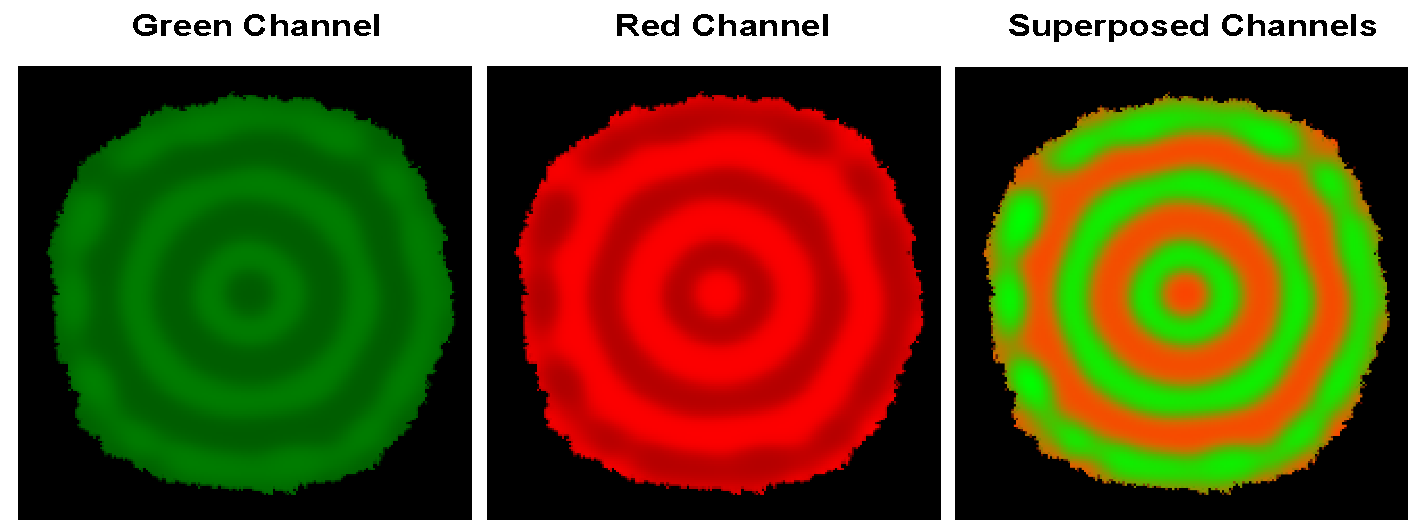
\includegraphics[width=1\textwidth]{chapters/Methods/redgreesupersposed}
    \caption{Flourescent channels from obtained from the simulation}
    \label{redgreesupersposed}
\end{figure}




\section{Experimental methods}
\subsection{Transformation through electroporation}\label{electroporation}
1 $\mu L$ of DNA containing the 4 plasmids was added to 25 $\mu L$ of electrocompetent MK01 \textit{E. coli} cells.
These four plasmids make up the full gene circuit seen in Fig.~\ref{fig:synthetic circuit_chapter2}.
Details of these plasmids are in~\ref{tab:plasmid table}.
This mixture was placed on ice for a minute before being transferred to an electroporation cuvette.
The cells were then electroporated at 100 $\Omega$, 25 $\mu F$, and 1.8 $kV$.
Post-electroporation, the cells were immediately suspended in 500 $\mu L$ of SOC medium inside the cuvette.
This suspension was then moved to an aeration tube and allowed to recover for 1h shaking at 37 $^{\circ} C$, 220rpm.
Finally, 100$\mu l$ of the culture was plated and grown in LB agar plates with the necessary antibiotics and grown overnight at 37 $^{\circ} C$.

\begin{table}[H]
    \centering
    \begin{tabular}{llll}
        \toprule
        \textbf{Plasmid} & \textbf{Resistance} & \textbf{Contains …} & \textbf{Copy number} \\
        \midrule
        \textbf{pCOLA} & Kan 50 & Node A & Medium (20 – 40) 21 \\
        \textbf{pCDF} & Spec 50 & Node B & Medium (20 – 40) 21 \\
        \textbf{pET} & Amp 100 & Node C & Medium (20 – 40) 21 \\
        \textbf{pCC1} & CA 10 & Regulator cassette & Single copy 22 \\
        \bottomrule
    \end{tabular}
    \caption{Circuit plasmids built by Dr. Jure Tica and Tong Zhu. Each circuit node is encoded in a different cassette.}
    \label{tab:plasmid table}
\end{table}


\subsection{Microscopy}\label{microscopy}
After electroporation, transformed cells were grown in 2xYT medium (Sigma-Aldrich Y1003) with the required antibiotics to an OD600 of 1.5. They were then diluted in fresh 2xYT by a factor of $10^4$.
6 well MatTek plates with glass coverslips on the bottom were used for imaging.
1.4\% (w/v) agar (Sigma-Aldrich A5306) was plated in the 5 wells containing the desired antibiotics and inducers on top of the coverslip.
The diluted cells were then added on the agar and spread with beads (Novagen 71013).
The plates were then sealed in parafilm to avoid drying out of the agar and covered in aluminium foil to prevent photobleaching of the fluorescent proteins (in case the signal of the emergent pattern is very weak).
The plates were then incubated at 37 $^{\circ} C$ for 4 days and imaged daily.
Colonies grew over time in the wells of the MatTek plates as shown in Fig.~\ref{matek}.

\begin{figure}[H]

    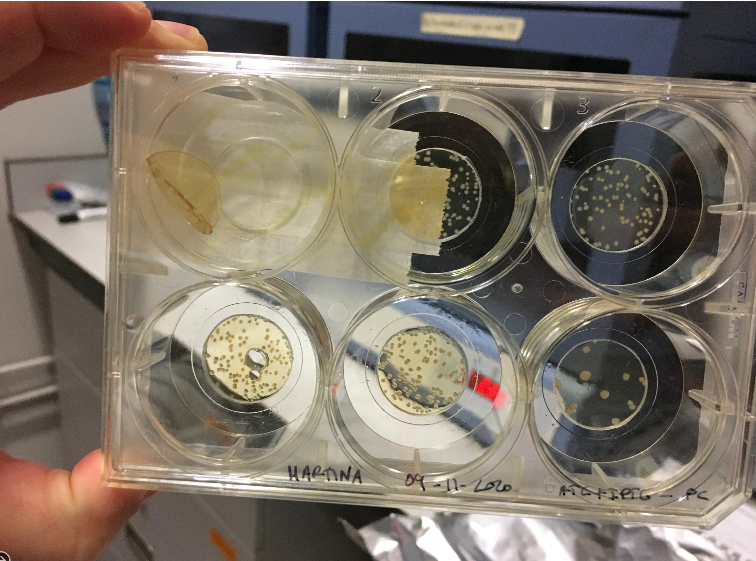
\includegraphics[width=1\textwidth]{chapters/Methods/matek}
    \caption{Bacterial colonies with synthetic gene circuit grown on 6-well MatTek plates.}
    \label{matek}
\end{figure}

These colonies were then imaged in the confocal Leica SP8 microscope with a 10x objective.
Confocal microscopy was carried out in the Facility for Imaging by Light Microscopy (FILM) at Imperial College London on a Leica SP8.
FILM is part-supported by funding from the Wellcome Trust and BBSRC.
More details of confocal imaging protocol including imaging parameters can be found in~\parencite{Tica2020}.

The opening and superposing of the confocal microscopy images is performed in Fiji (ImageJ v2.1.0).
None of the images are subjected to post-processing by linear or non-linear colour map transformations.

